\begin{figure*}[t!]
\centering
\begin{subfigure}[h]{\textwidth}
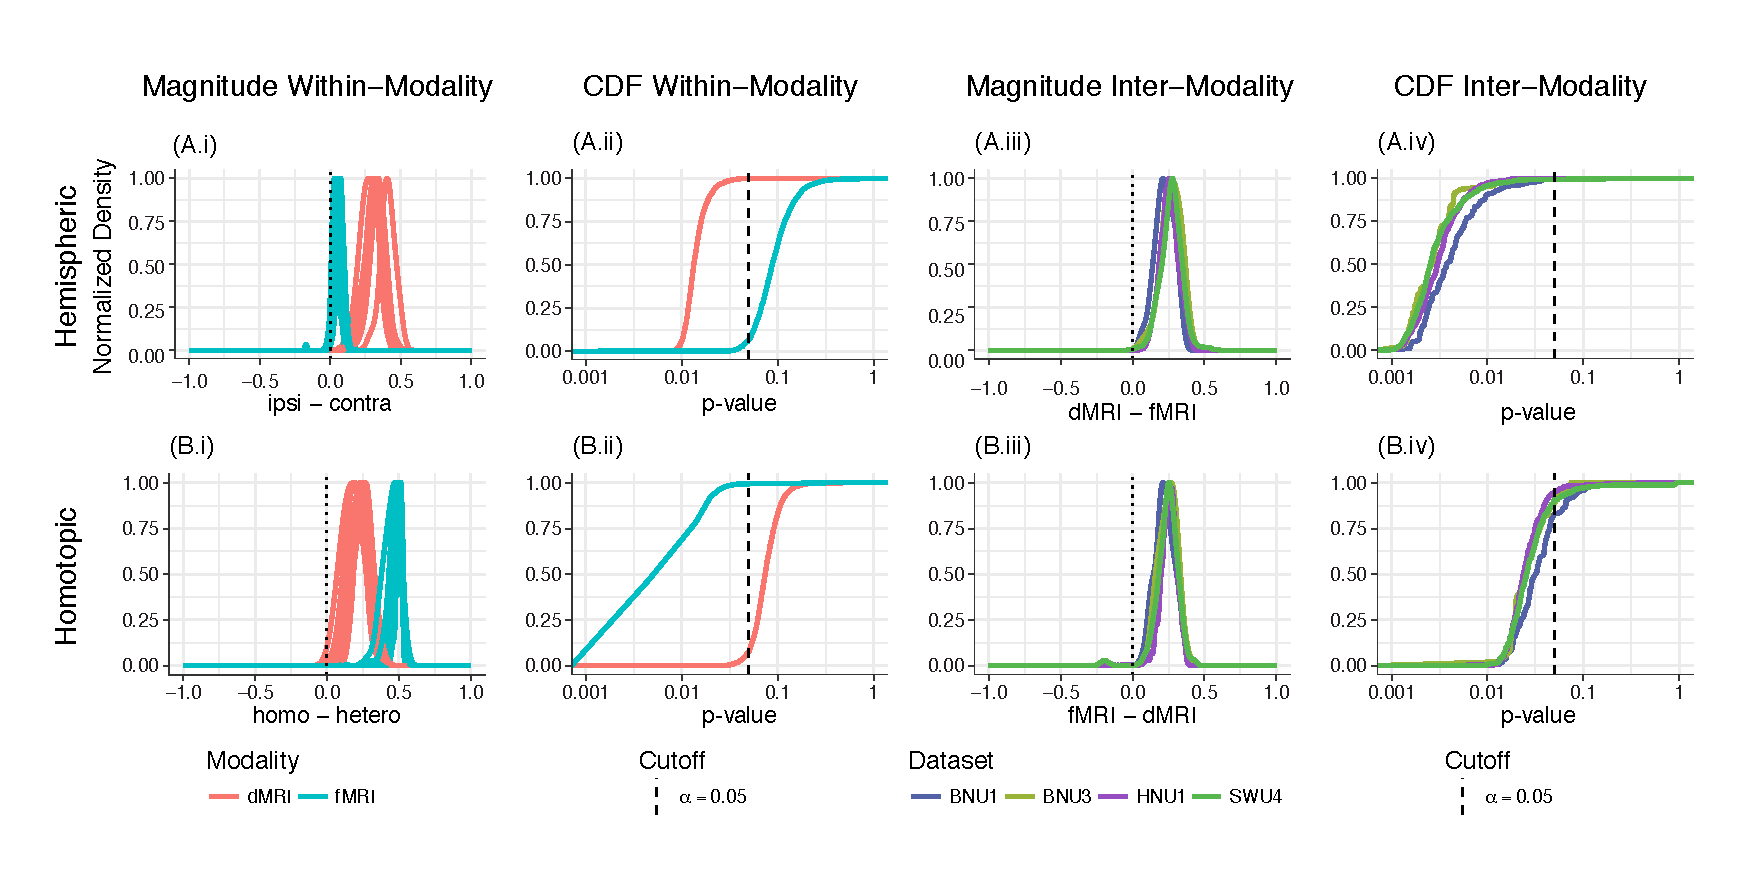
\includegraphics[width=\textwidth]{./figs/figure_siem.pdf}
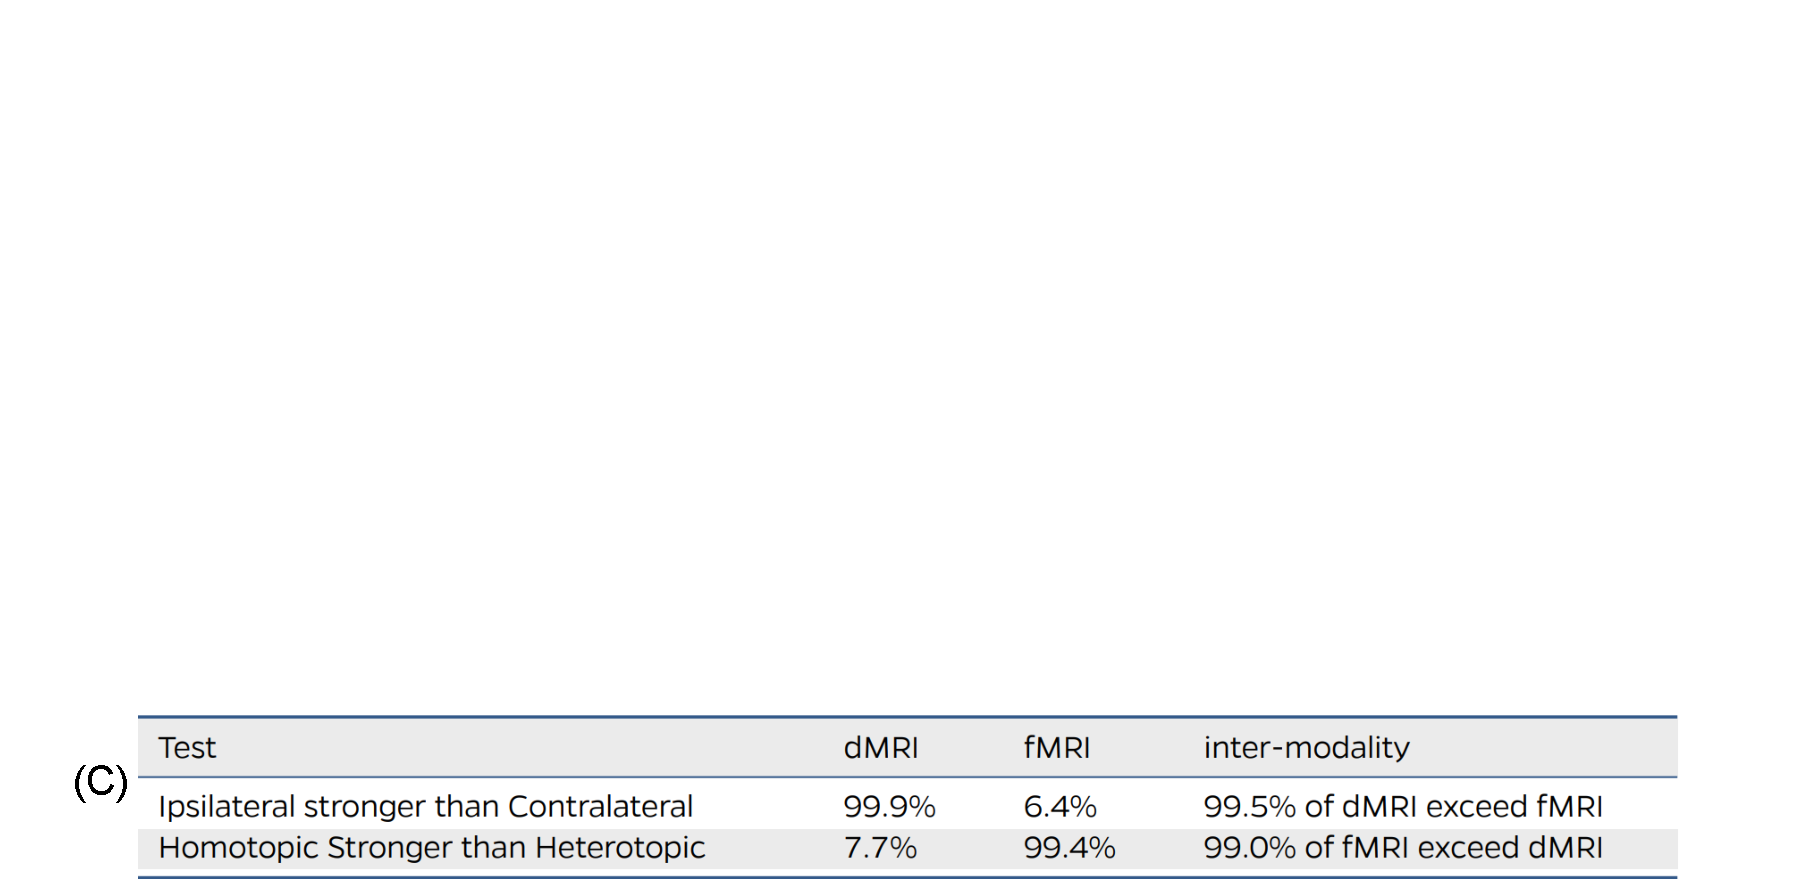
\includegraphics[width=\textwidth]{./figs/table_siem.pdf}
\end{subfigure}
\caption{\textbf{Structured Independent Edge Model  (SIEM) establishes multi-connectome properties are preserved both within and across studies}.
\textbf{(A.i)} The magnitude of the difference indicating whether ipsilateral (within hemisphere) connections differ from contralateral (across hemisphere) connections. The dMRI connectomes appear to have a greater connectivity difference than fMRI connectomes.
\textbf{(A.ii)} The distribution of p-values indicating whether ipsilateral connections are significantly stronger than contralateral connections, on average.  Essentially every dMRI connectome yields significantly stronger ipsi- than contralateral connectivity, whereas essentially no fMRI connectome does.  
\textbf{(A.iii)} For four studies with both dMRI and fMRI, one can compare connection strengths across modalities for a particular individual. The ipsi-versus-contra discrepancy in the dMRI exceeds that of the fMRI.
\textbf{(A.iv)}  In essentially all sessions, dMRI has a significantly stronger within-versus-across discrepancy of connection strength than the corresponding fMRI connectome in most of same-individual pairs. 
\textbf{(B.i)} Same analysis comparing homo- to heterotopic connections, indicating that the fMRI connectomes appear to have a greater connectivity difference than the dMRI connectomes.
\textbf{(B.ii)} fMRI exhibits significantly stronger homotopic connections, whereas dMRI does not.
\textbf{(B.iii)} Same approach as (A.iii), the homo-versus-hetero discrepency in the fMRI exceeds that of the dMRI.
\textbf{(B.iv)} fMRI has a significantly stronger homo-versus-hetero discrepancy of connection strength than the  corresponding dMRI connectome. 
% of the intra-modality per-graph $p$-values that ipsi-lateral connectivity exceeds contra-lateral connectivity,  one line per site. Low $p$-values indicate that  ipsilateral connectivity is significantly stronger than contralateral.  ~\textbf{(C)} the density estimates of the inter-modality 2-graph $p$-values that this difference in connectivity is stronger in the dMRI connectomes for a particular individual than in the fMRI connectomes for that individual. One line is reported per dataset indicated in the legend. Low $p$-values indicate that we are less-likely to falsely report a difference in connectivity in dMRI connectomes vs. fMRI connectomes. $99.5\%$ of the graph-pairings exhibit this property. \textbf{(B)} the density estimates of the per-graph $p$-values that homotopic connectivity exceeds heterotopic connectivity. Low $p$-values indicate that we are less-likely to falsely report a difference in connectivity homotopically  vs. heterotopically. $99.4\%$ of the fMRI connectomes exhibit this property, whereas only $7.7\%$ of the dMRI connectomes exhibit this property. ~\textbf{(D)} the density estimates of the 2-graph $p$-values that this difference in connectivity is stronger in the fMRI connectomes for a particular individual than in the dMRI connectomes for that individual. Low $p$-values indicate that we are less-likely to falsely report a difference in connectivity in fMRI connectomes vs. dMRI connectomes. $99.0\%$ of the graph-pairings exhibit this property.
\textbf{(C)} Table showing fraction of individuals exhibiting significance effects of each analysis described above, demonstrating consistency across individuals and studies.}
\label{fig:siem}
\end{figure*}